\documentclass[a4paper]{article}
%\usepackage{fourier-otf}
\usepackage[utf8]{inputenc}
\usepackage{graphicx}
\usepackage{amsmath}
\usepackage{amsfonts}
\usepackage{float}
\usepackage{biblatex}
\addbibresource{bibliography.bib}
\usepackage{listings}
%\usepackage[square,sort,comma,numbers]{natbib}
\newtheorem{theorem}{Theorem}[section]
\usepackage{color}
\usepackage{makeidx}
\usepackage{titlepic}
\definecolor{mygreen}{rgb}{0,0.6,0}
\definecolor{mygray}{rgb}{0.5,0.5,0.5}
\definecolor{mymauve}{rgb}{0.58,0,0.82}
\lstset{ %
	backgroundcolor=\color{white},   % choose the background color
	basicstyle=\footnotesize,        % size of fonts used for the code
	breaklines=true,                 % automatic line breaking only at whitespace
	captionpos=b,                    % sets the caption-position to bottom
	commentstyle=\color{mygreen},    % comment style
	escapeinside={\%*}{*)},          % if you want to add LaTeX within your code
	keywordstyle=\color{blue},       % keyword style
	stringstyle=\color{mymauve},     % string literal style
}
\usepackage{hyperref}
\hypersetup{
  colorlinks   = true,    % Colours links instead of ugly boxes
  urlcolor     = black,    % Colour for external hyperlinks
  linkcolor    = black,    % Colour of internal links
  citecolor    = black      % Colour of citations
}
\title{First chapter}

\author{F.Bernardi}







\begin{document}
		\maketitle
		
		\begin{minipage}{\linewidth}
			\centering
			\begin{minipage}{0.45\linewidth}
				\begin{figure}[H]
					
\includegraphics[width=\linewidth]{Logo_IIT.png}
					
				\end{figure}
			\end{minipage}
			\hspace{0.05\linewidth}
			\begin{minipage}{0.45\linewidth}
				\begin{figure}[H]
					
\includegraphics[width=\linewidth]{Logo_Politecnico_Milano.jpg}
					
				\end{figure}
			\end{minipage}
		\end{minipage}
	
	\clearpage
	
	\clearpage
	
	\section{Introduction}
	
	
	In this first chapter, the biological and experimental foundations of this work will be presented. After a brief review of the main notions of neurobiology, such as the structure of a neuron, the propagation of an action potential in neuronal circuits and the intracellular calcium dynamics, there will be a closer focus on the areas of the brain interested in the following discussions.\\
	The final part consist in the description of the behavioral tasks performed on mice and the experimental techniques for calcium imaging, which constitute the source of the analyzed data in the following chapters.
	
	\subsection{Neurobiology of emotions and behaviour}
	
	\begin{figure}[H]
		\begin{center}
			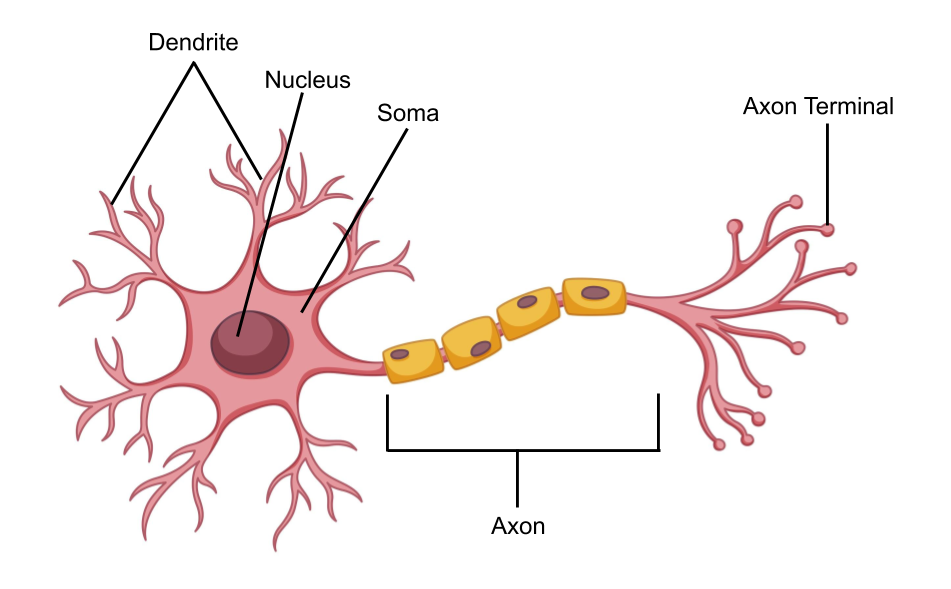
\includegraphics[scale=.25]{neuron.png} 
		\end{center} 
		\caption{\textit{Schematic representation of a neuron}}
		
	\end{figure}
	
	The importance of the brain in mammals is more evident day by day: it allows us to think,  to capture the stimuli from the environment, elaborate them to then enrich our memory and  our learning. It is the control center of our movements and our actions, it allows us to speak, to understand other individuals and elaborate reesponses. Most importantly for this work, however, The brain, from its basic cellular units, can explain our behaviour and our emotions. \\
	
	The brain itself is part of the \textbf{nervous system (NS)}, and its most important cell is the \textbf{neuron}: it is the basic unit needed for the transmission of the electrical signal, both within the same area and between different areas of the organism, allowing the body to collect informations, react to stimuli and make decisions based on them. \\
	The neuron is composed by a central body called \textit{soma}, where all the cellular functionalities happen, by the \textit{dendrites}, cellular extensions which collects stimuli from near areas, and \textit{axon}, the biological cable connecting one neuron to another, in order to propagate informations. 
	The second type of cells present in the NS are the \textbf{glial cells} (like astrocytes) , which perform functions of protection, susteinment and nutritions for the neurons. Altough they won't be treated in this work, their contribution should not be neglected, as it has been shown to be relevant in many important processes fo the nervous system [Semyanov, Henneberger 2020]. \\
	
		
	
	Neurons are \textbf{eccitable} and \textbf{conducible}, i.e. they can generate an electrical impulse and trasmit it to other neurons, forming neuronal microcircuits, often associated to a specific area and/or task. \\
	Inside every neuron, in the cytoplasm, there is a cohexistence of different ionic species (mostly $Na^+, Cl^-, K^+, Ca^{2+}$) which, in equilibrium conditions, assume a certain concentration, determining itself a difference between the potential assumed inside and outisde the cell: we call this quantity the \textbf{membrane potential} of the cell (indeed it is the potential formed across the cell's membrane).  In reaction to an external stimulus, the ionic concentrations change rapidly their values, provoking a heavy change in the the membrane potential: here the eccitation of a neuron happens, as well as the formation of an \textbf{action potential}, which will propagate to other neurons across the axon. 
\begin{figure}[H]
	\begin{minipage}{\linewidth}
		\centering
		\begin{minipage}{0.45\linewidth}
			\begin{figure}[H]
				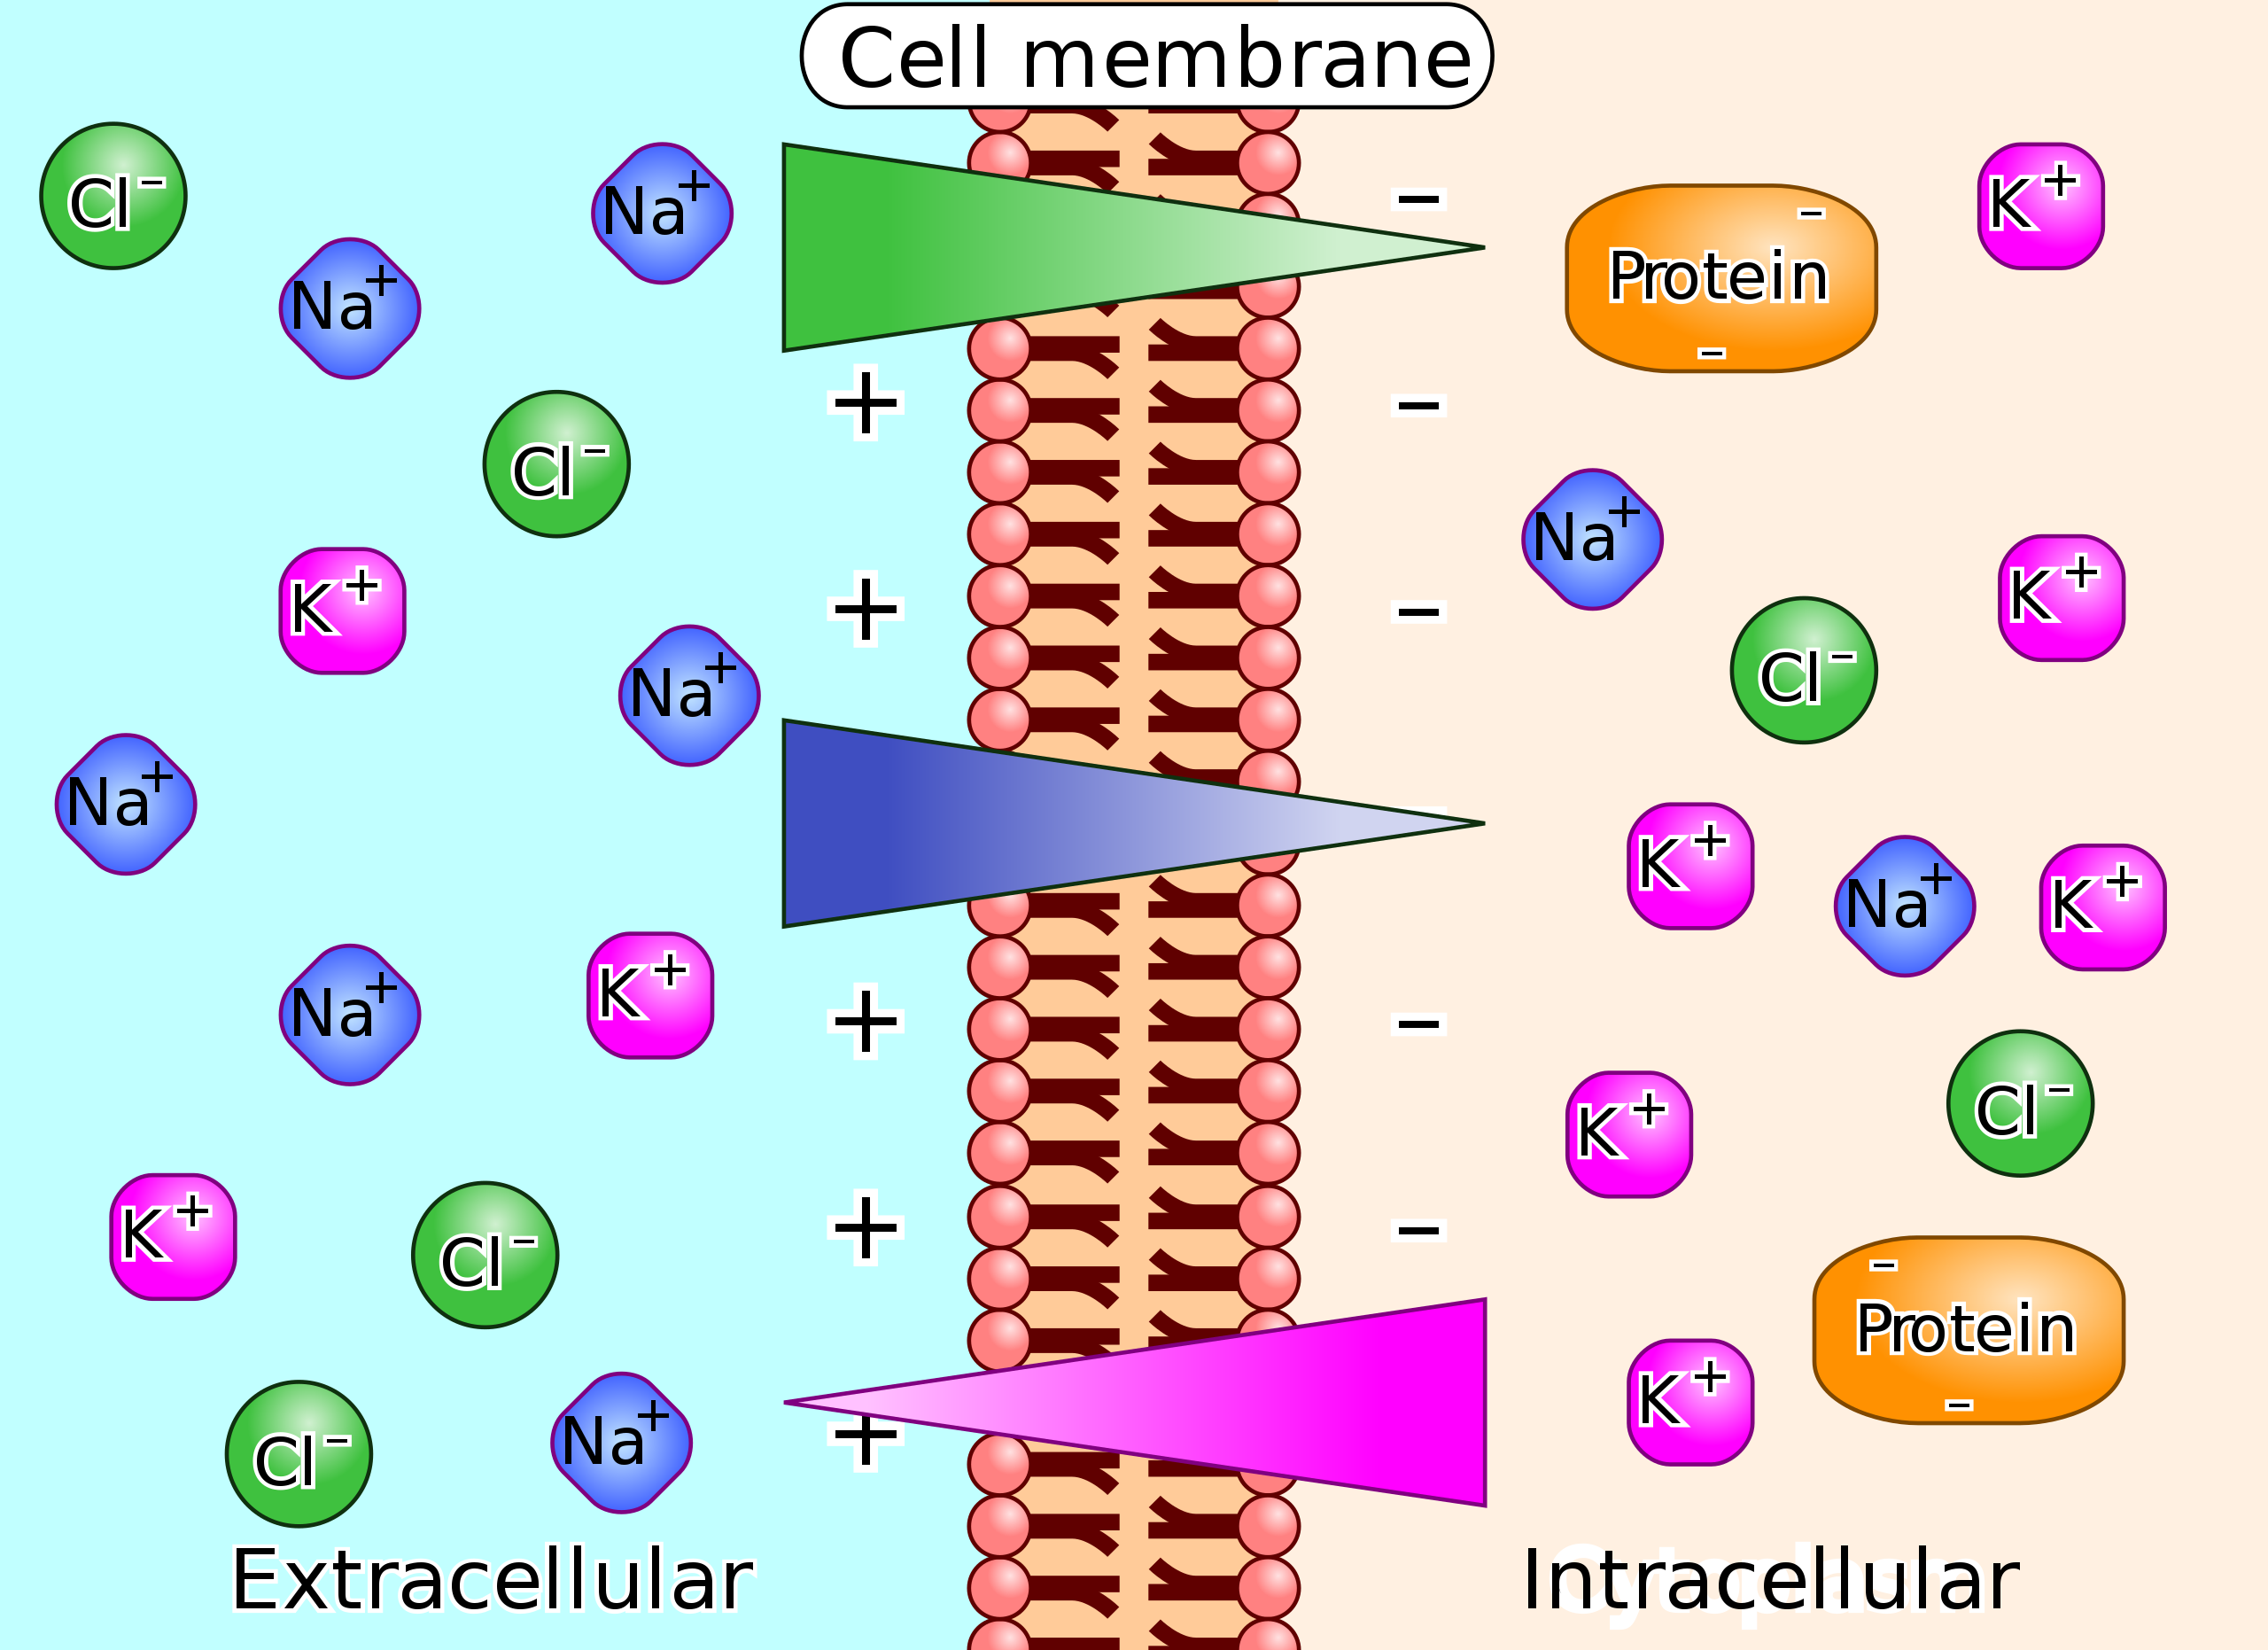
\includegraphics[width=\linewidth]{AP1.png}
				
			\end{figure}
		\end{minipage}
		\hspace{0.05\linewidth}
		\begin{minipage}{0.45\linewidth}
			\begin{figure}[H]
				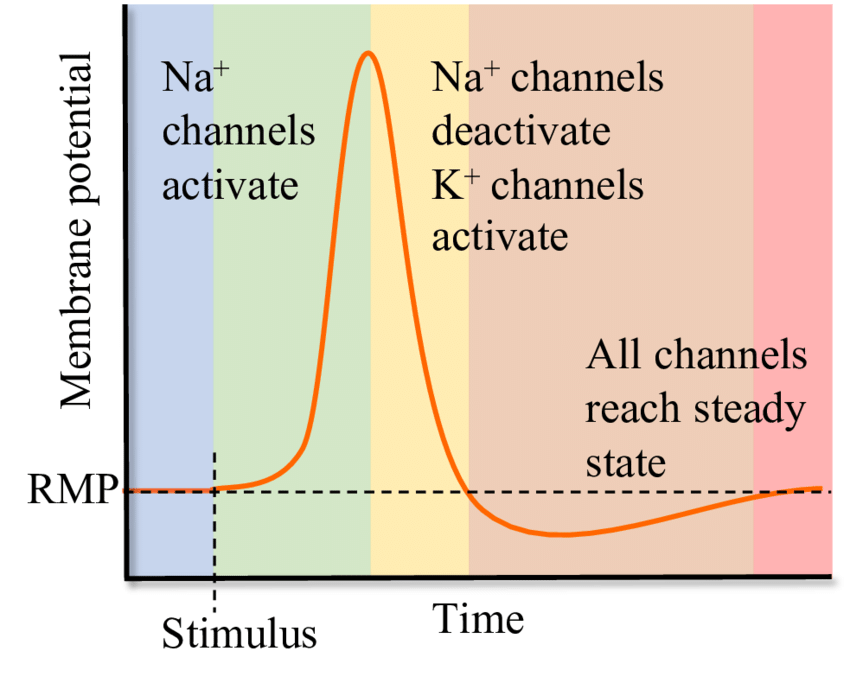
\includegraphics[width=\linewidth]{AP2.png}
				
			\end{figure}
		\end{minipage}
		
	\end{minipage}
\caption{\textit{Left: schematic representation of ionic species inside and outside the cellular membrane. Such species are allowed to pass through the membrane only in specific circumstances through adhibited ionic gates \\
Right: example of action potential formation in reaction to a stimulus}}
\end{figure}

At the end of the axon, the link between a neuron and its neighboor, and the relative passage of the electrical impulse, happes thanks to a chemical \textbf{synapse}. In the terminal of the axon, special molecules called \textit{neurotransmitters} are sintethized, and the arrival of an action potential allows such molecules to travel towards the \textit{intersynaptic space}, where they can bind to receptors located in the post-synaptic cell. The response of the post-synaptic cell, then, can be either excitatory or inhibitory, based on whetever the impulse is preserved in the circuit or supressed.\\
The synapse (and its correspondent neuron) can be calssified in four main groups, depending on the type of neurotransmitter which they release:  glutamatergic, GABAergic, , cholinergic,  adrenergic. The most relevant for this work will be the GABAergic, consisting of inhibitory neurotransmitters reducing the excitability of the neurons.
\begin{figure}[H]
	\begin{center}
		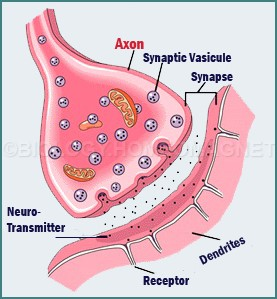
\includegraphics[scale=1.6]{synapse.jpg} 
	\end{center} 
	\caption{\textit{Schematic representation of a chemical synapse}}
	
\end{figure}



In neurobiology, the conditions under which a neuron can be considered \textbf{active} are not unique and matter of debate; in general, however, when talking about neural activity, the literature usually means either the already discussed electrical activity, either the \textbf{calcium activity}. The intracellular dynamic of this particular element, in ionic form of $Ca^{2+}$, is known to be essential for the main cellular proccesses, and it is strictly related to the formation of an action potential and subsequent propagation of the elctrical impulse.\\
 Indeed, we can usually observe a \textit{strong instabilities} in the intracellular calcium concentration values, which often show fast oscillations and changes, through the formation of sudden peaks: we will define the neuron as \textit{active} in correspondence to this peaks.

\begin{figure}[H]
	\begin{center}
		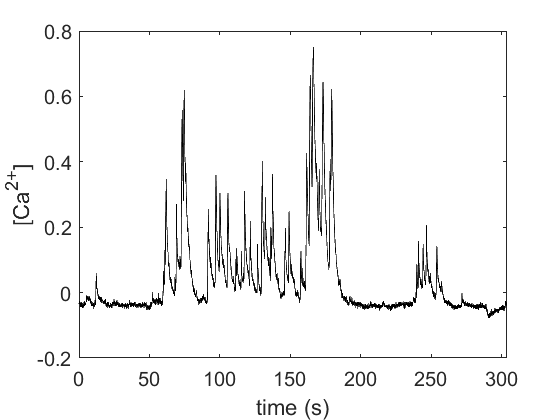
\includegraphics[scale=.50]{Ca_conc.png} 
	\end{center} 
	\caption{\textit{Example of $Ca^{2+}$ concentration recorded in a neuron, as function of time}}
		
	\end{figure}
	
	Once defined the meaning of neuronal activity, we can ask ourselves wether this activity could be related to aspects like behaviour, emotion, body language, mood: in other words, to investigate wether there is a connection between the activation of some specific neurons, and what animals feel or do.\\
	This topic has fascinated neuroscientist for decades, and from it has been discovered so far, it seems evident that \textbf{different areas of the brain are responsible for different emotions, feelings or behaviours} (altough this distinctions may not always be that marked, unique and easy to detect).

	
	The neurobiology experiments on which this work relies on refer mainly to some particular areas of the brain, which previous studies found to be strictly connected to emotional processes [Etkin et al. 2011]:
	\begin{itemize}
		
		\item \textbf{Medial prefrontal cortex (mPFC)}:  part of the frontal cortex, the are of the brain situated in the frontal lobe. This area is implicated in cognition processes like emotional or social, but strong connections with decision making have been found as well[Carlen 2017]
		
		\item \textbf{Anterior Cingulate Cortex (ACC)}: part of the cingulate cortex and situated in proximity of the mPFC,  of which the ACC shares a lot of functionalities. Indeed, experimental evidences of the connection between this area of the brain and emotions have been found [Zheng 2020]. This area seems also to be implicated in social aspects like morality or empathy [Carillo 2019], as reaction to interactions with another individual
		
		\item \textbf{Amygdala}: nuclear complex located in the medial part of the temporal lobe. It is responsable for the elaboration of the emotions, it collects stimuli from the talamus and elaborate responses: in other words, it's a sort of emotional thermometer of the body and the decision maker for adeguate responses [ARTICOLO?]
	\end{itemize}


	
	\begin{figure}[H]
		\begin{center}
			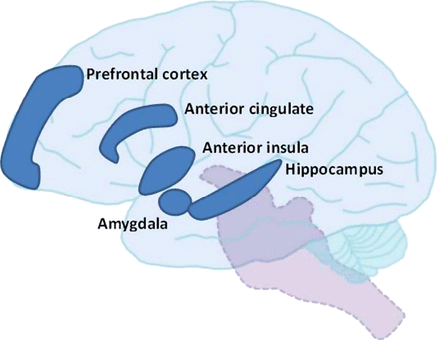
\includegraphics[scale=.55]{brain.png} 
		\end{center} 
		\caption{\textit{Main areas of the brain involved in behavior and emotion recognition}}
		
	\end{figure}

\newpage

\subsection{In vivo studies on mice}

According to the \textit{Foundation of Biomedical Research (FMR)}, approximately $95\% $ of all lab animals are mice or rats, as it is in the case of this current work. Altough very often the final goal of the research is an application useful for humans, the reasons why mice are the first choice for experiments are numerous: first of all, mice are mammals quite similar to humans when it concerns genetic, at the point that scientists have been able to reproduce genes in mice similar to the ones implied in human deseas ("\textit{transgenic mice}" [Harari,Abramovich 2014]); rodents, indeed, are also easy to manipulate from a geentic point of view. Another reason is surely the convenience: mice are small, easy to control, quite cheap to buy and usually docile. Finally, being the most used animal in research, the largest informations and literature which can be found is about them, their anatomy, their typical behaviours, and by today large populations of rodents have been created and used exclusively for experimental purposes, being almost all identical between them and therefore setting a uniform standard for study and validation of results. \\
Through a  \textbf{behavioral task}, one or more mice are put in a particular situation created to study their reactions, such as a shown behaviour or movement, and, in this context, the goal is to find a relationship with their correspondent neural activity. Therefore, the overall experiment consist in the following steps:
\begin{enumerate}
	\item Preparation of the arena and equipment for the task 
	\item Preparation of the mice to the experiment, both in term of behavioral condiitoning, both for neural acitvity measurments
	\item Performance of the test with simultaneous recordings of  aspects of interest such as behavior or neuronal activity
	\item Pre-processing and analysis of the collected data
\end{enumerate}

\begin{figure}
	\begin{center}
		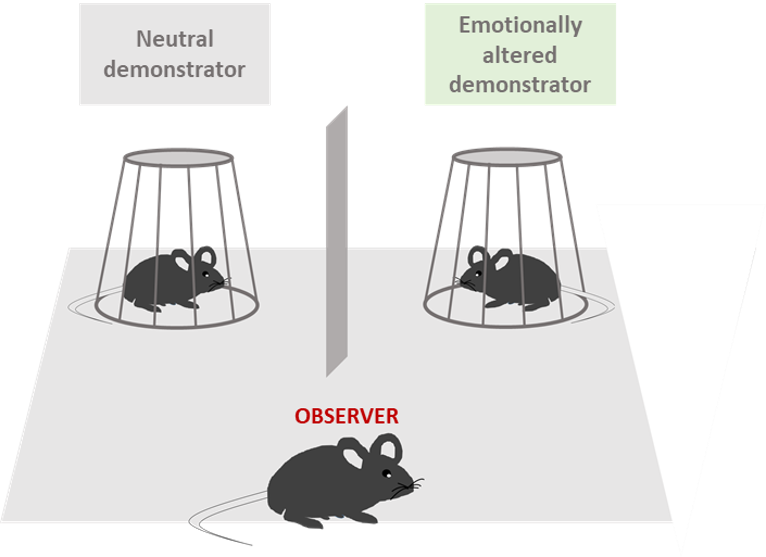
\includegraphics[scale=.60]{mice_task.png} 
	\end{center} 
	\caption{\textit{Basic setting of the emotion discrimination task: one mouse (the \textit{observer}) is free to move in the arena, while the others two (the \textit{demonstrators}) remain inside a cage. One of the demonstrators has a neutral affective state, the other an altered affective state}}
	
\end{figure}
In this work, the behavioral task which has been studied is a particular realization of the \textbf{emotion discrimination task}. The first step of these type of tasks, performed in this way other times in the past, consists in the presence of three mice: one, called the \textit{observer}, is a mouse freely to move in an arena, while the others, the \textit{demonstrators}, remain in a cage. In the phase preceding the test, the \textit{habituation phase}, one of the two demonstrators is \textbf{emotionally altered}: namely, it is subjected to specific conditions and procedures which provoke an alteration of his affective state. This alteration could be either negative (usually stress condition following a period of water deprivation) or positive (usually relief condition, consisting in water \textit{ad libitum} following water deprivation). The other demonstrator, such as the observer, is instead in a \textit{neutral} state.\\

Previous works on this setup [Scheggia-Managò] were performed using both positive and negative affected demonstrators. The cellular target consisted in a specific subpopulation of neurons, which is thought to be involved in processes like \textit{affective state discrimination}: the SOM+ internuerons in the medial prefrontal cortex.\\
These neurons, expressing the \textbf{somatostatin} neurotransmitter, form a small group compared to others like \textit{piramidal neurons} or \textit{parvalbumin neurons}, but unlike these former ones, they seem to be directly implicated in the affective state discrimination of a conspecific. The data analysis on the task showed some remarkable results:

 \begin{itemize}
 	
 	\item The time spent by the observer near the altered demonstrator was significantly higher than the one spent near the neutral one, such as the moments when reciprocal sniffing between two close mice happened
 	
 	\item This  discrimination appears to be stronger in the first period of the test
 	
 	\item The discrimination is directly connected to the present of a mouse in aletered state, since from the repeatition of the task with two neutral demonstrators, no significant differences emerged
 	
 	\item The neural activity of the observer (both in term of electrical impulse and  calcium peaks) showed stronger values during the interactions with the altered mouse rather than the neutral
 	
 	\item  If a mechanism of \textit{optical inhibition} of SOM+ cells [REFERENCE?] is performed before the test, the discrimination disappears, namely no relevant differences between time spent, sniffing and neural activity have been observed with altered demonstrator rather than the neutral
 	
 	\item All the previous considerations do not apply to other neuronal categories like piramidal or parvalbumin interneurons
 	 
 \end{itemize}
 
 Overall, these results seems to show a \textbf{key role of the somatostatin interneurons in affective state discrimination}.

	\begin{figure}
	\begin{center}
		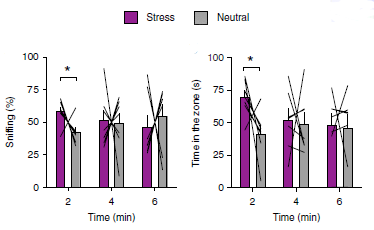
\includegraphics[scale=.99]{scheggia.png} 
	\end{center} 
	\caption{\textit{Recording of sniffing times (left) and vicinance times (right) between observer mouse and stressed demonstrator}}
	
\end{figure}


Targeting this specific neuronal subpopulation, The hope is to find always more evidences on its link with a proper showed tendency, emotion or behavior. In the case of the discussed task targeting SOM+ interneurons in the mPFC, for example, the observed effects in the abolition of discrimination, through photonibition of such neurons, could be similar to the ones observed in neurodegenerative disorders such as autism spectrum disorders (ASDs) or schizophrenia. Therefore, this approach aims to investigate the causes of a specific behavior at a basic and detailed level such the one of single neuron precision. \\
In order to do so, The paradigm of the task has to be defined in a way that it allows a collection of unbiased results, but an adeguate way to perform an imaging of the neuronal activity of interest is necessary as well and described in the following sectrion. As final step, a proper data analysis on those results has to be performed (chapter 2).

\newpage
\subsection{Calcium imaging through Inscopix}



\begin{figure}[H]
	\begin{center}
		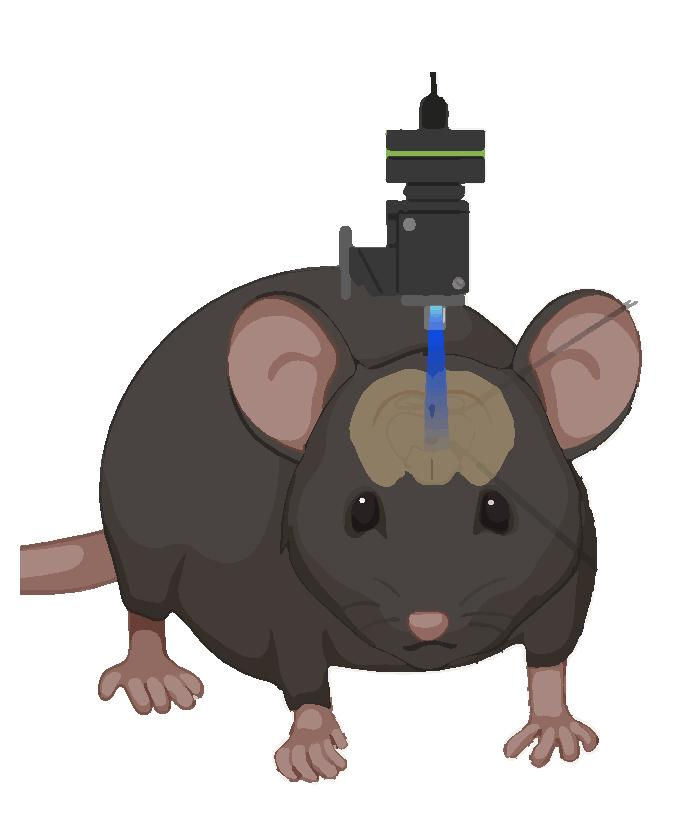
\includegraphics[scale=.35]{Inscopix.jpg} 
	\end{center} 
	\caption{\textit{The Inscopix miniscope}}
	
\end{figure}


In this section, a powerful tool for single neuron calcium imaging will be presented. The Inscopix company [REF TO INSCOPIX] provides tools and software to extract calcium tracks as one photon measurements from in vivo experiments on mice.\\
To measure the intracellular $Ca^{2+}$ concentration in a single mouse during a behavioral task, the first step is the performance of a surgery on the mouse to implant a miniscope in the \textit{region of interest (ROI)} of the brain. On the same mouse, \textbf{genetically encoded calcium indicators (GECI)}, such us the \textbf{GCaMP} protein, are adopted. These type of proteins, when bound to $Ca^{2+}$, emit a fluorescent light, which intensity will be captured by the miniscope. At the end of the test, the miniscope will be able to give back a video of the ROI, in which the evolution of the fluorescence through time can be appreciated  in the neurons. In this way, we have a representation of the intracellular calcium oscillations behaviour during the whole task. These informations will be combined with behavioral or positional data of the mice in the arena, making possible to start a data analysis and look for correlation between behavior and neural activity.\\
In order to have the data ready to be analized, however, the Inscopix software manage also the pre-processing part, which goes through the following steps:

\begin{enumerate}
	
	\item If needed, more videos recorded from the test are combined, in order to obtain a single final video of the ROI through time
	
	\item \textbf{Spatial and temporal downsampling} are performed, selecting the appropriate scale factors of space and time which allow to capture all the important intels
	
	\item \textbf{Spatial filtering} of the image: it removes low and high frequencies with a bandpass filtering. The filter has the form
	
	$$ M_f^{band} = GB(M_f,\sigma_{high}) - GB(M_f,\sigma_{low})$$
	
	Where $M_f$  represents the frame $f$ of movie $M$, $GB$ is the \textit{Gaussian Blur} function, and the standard deviations $ \sigma_i = \frac{2 ln(2)}{2 \pi \lambda_i}$ are computed from the cut-off values $ \lambda_{high}$ and $ \lambda_{low}$
	
	\item \textbf{Motion correction}: it accounts of the motions between different frames of the videos, applying a correction to let every pixel staying at the same place in different frames
	
	\item \textbf{Pixel normalization}: each pixel of a frame represents a different luminosity, caused by the fluorescence in reaction to the GCaMP. After the preprocessing, the value of the fluorescence (which estimates the calcium concentration) is expressed as 
	$$\frac{\Delta F }{F} = \frac{F(x,y,t) - F_b}{F_b}$$
	where $F(x,y,t)$ represents the measured fluorescence in the point $(x,y)$ at time $t$, while $F_b$ is a baseline fluorescence value (usually the mean value of the movie, in some cases the minimum). aAter this step, the returned value for every pixel is an adimensional relative value of fluorescence
	
	\item The \textbf{PCA-ICA algorithm} attempts to recognize the neurons of the ROI in the movie. Based on given informations such as average cell's diameter, an indipendent component analysis is done, followed by a principal component one, until convergence. In particular, the frames of the movie, represented as matrices, are rasterized into 1D vectors and they are normalized on mean and standard deviation. At this point, a principal component analysis is performed, in order to reduce dimensionality. Every frame is then approximated by a weighted sum of the principal trace components. Finally, an ICA algorithm is launched. At the end of this process, every neuron will be identified, labeled, and gifted with a calcium activity values (which is actually a $\frac{\Delta F }{F}$ value) for every time stamp of the movie. 
	
	\item \textbf{Final adjustements}: appropriate algorithms or manual fixing are done to take into account some imperfections like mistakes in neuron identification, imprecisions due to overlapping regions, excessive noise in the calcium traces for a neuron (discarding the correspondent cell from the analysis)
	
	\item \textbf{Data import}: finally, data are imported in a csv file. Therefore, the final data available consist in a list of every neuron detected and their correspondent value of $\frac{\Delta F }{F}$ recorded at every time stamp
	
\end{enumerate} 
	
\begin{figure}[H]
	\begin{center}
		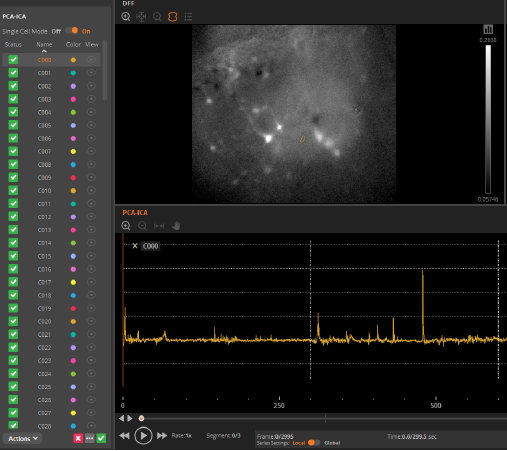
\includegraphics[scale=.70]{Inscopix2.png} 
	\end{center} 
	\caption{\textit{Example of pre-processing work through Inscopix software. We can appreciate: the list of detected neurons (left), a segment of the video in the ROI (top-right) and an example of the calcium track recorded in a single neuron through time (bottom-right)}}
	
\end{figure}

\newpage
\subsection{Calcium imaging through Fiberphotometry}

\begin{figure}[H]
	\begin{center}
		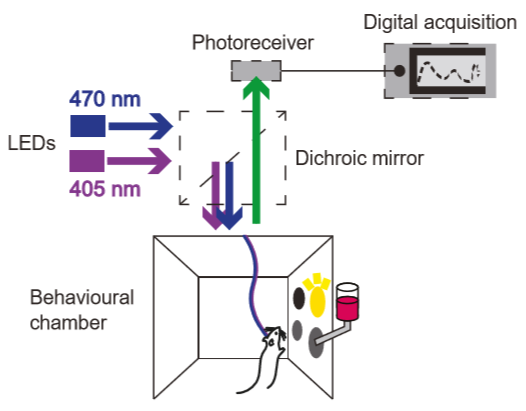
\includegraphics[scale=.50]{fiberphotometry.png} 
	\end{center} 
	\caption{\textit{Fiberphotometry experimental setup}}
	
\end{figure}

In the previous section it has been shown a calcium imaging technique based on single neuron traces measured with single photon miniscopes. In this section, another common technique for calcium imaging will be presented: \textbf{fiberphotometry}. \\
The main goal of this technique is the same of the Inscopix imaging one, however technical equipment, methodology and results present substantial differences.\\
Relying on genetically encoded calcium idicators such as GCaMP, with fiberphotometry the fluorescence signal is recorded thorugh \textit{optic fibers}, typically of length $300-400 \mu m$. An excitation of GCaMP is performed using a blu LED light at the approriate wavelength ($470 nm$), which is transmitted through the optical cannula implanted in the mouse, while an emission green light ($525 nm$) is relayed to a photoceiver. Often, a second excitation light (violet, $405 nm$), is used as well, to take into account autofluorescence and produce an isosbestic control signal [TESI PHD GIULIA].\\
 Finally, a software manages the output signal in order to perform filtering and give out a collective raw signal, separating the two contributions from blu and violet lights. Such signal, in contrast with the miniscope neuronal imaging, can only be an \textit{aggregate} signal of the observed area. This implies that the fiberphotometry technique produces signals at smaller spatial resolution than the previously introduced technique. However, this technique is becoming always more used because the smaller accuracy is compensated by several positive factors:

\begin{itemize}
	
	\item The overall experimental setup for fiberphotometry results cheaper than the one for miniscope imaging 
	
	\item The procedure operated in mice are less invasive, and the subjects are more suitable to long freely behaving experiments
	
	\item The implant of the cannula is relatively easy to perform, and a good signal is collected even with fiber pacements in the neighborhood of GECI -expressing populatiobs [Siciliano and Tie 2018]
	
	\item Multiple areas of the brain can be investigated at same time 
	
	\item Fiberphotometry can be used for others fluorescent indicators, such as norepinephrine (Feng et al., 2019), GABA (Marvin et al., 2019), glutamate (Liang et al., 2015),
	acetylcholine (Jing et al., 2018) and dopamine (Patriarchi et al., 2018)
	
	
	
\end{itemize}


\subsection{Synchronization of neural activity}




\end{document}




\section{Introduction}

\begin{figure}[H]
\begin{center}
	\includegraphics[scale=.40]{ad_stab.png} 
\end{center} 
\caption{\textit{Numerical solution (blu) and real solution (black) in the  stabilized case for advection-diffusion problem}}

\end{figure}